\section{Climate Forcing}

Something about climate forcing options for GLIMMER-CISM. Essentially, this include EISMINT and GLINT, and the SMB schemes, which we are unfamiliar with. I'm lumping them all in here simply 
because they have something to do w/ climate and running the model. Other ``drivers" and climate forcing stuff that we don't support anymore has been commented out of this build.

%________________________________________________
%________________________________________________
%
%	EISMINT "driver" (does this exist anymore?) described here
%________________________________________________
%________________________________________________


\subsection{EISMINT Driver}\label{driver:eismint}

** Note sure if this even formally exists. I'm guessing this is called during the EISMINT test cases, but if there is no obvious way for someone to ``get" at it, I wonder if 
we need to bother describing in detail here. Oddly, this only talks about EISMINT 1. **

\subsubsection{Configuration}

\begin{center}
  \tablefirsthead{%
    \hline
  }
  \tablehead{%
    \hline
    \multicolumn{2}{|l|}{\emph{\small continued from previous page}}\\
    \hline
  }
  \tabletail{%
    \hline
    \multicolumn{2}{|r|}{\emph{\small continued on next page}}\\
    \hline}
  \tablelasttail{\hline}
  \begin{supertabular*}{\textwidth}{@{\extracolsep{\fill}}|l|p{11cm}|}
%%%% EISMINT-1 fixed margin
    \hline
    \multicolumn{2}{|l|}{\texttt{[EISMINT-1 fixed margin]}}\\
    \hline
    \multicolumn{2}{|p{0.95\textwidth}|}{EISMINT 1 fixed margin scenario.}\\
    \hline
    \texttt{temperature} & (real(2)) Temperature forcing $$T_{\mbox{surface}}=t_1+t_2d$$ where $$d=\max\{|x-x_{\mbox{summit}}|,|y-y_{\mbox{summit}}|\}$$\\
    \texttt{massbalance} & (real) Mass balance forcing \\
    \texttt{period} & (real) period of time--dependent forcing (switched off when set to 0) $$\Delta T=10\sin\frac{2\pi t}{T}$$ and $$\Delta M=0.2sin\frac{2\pi t}{T}$$\\
    \hline
%%%% EISMINT-1 moving margin
    \hline
    \multicolumn{2}{|l|}{\texttt{[EISMINT-1 moving margin]}}\\
    \hline
    \multicolumn{2}{|p{0.95\textwidth}|}{EISMINT 1 moving margin scenario.}\\
    \hline
    \texttt{temperature} & (real(2)) Temperature forcing $$T_{\mbox{surface}}=t_1-t_2H$$ where $H$ is the ice thickness\\
    \texttt{massbalance} & (real(3)) Mass balance forcing $$M=\min\{m_1,m_2(m_3-d)\}$$ where $$d=\sqrt{(x-x_{\mbox{summit}})^2+(y-y_{\mbox{summit}})^2}$$\\
    \texttt{period} & (real) period of time--dependent forcing (switched off when set to 0) $$\Delta T=10\sin\frac{2\pi t}{T}$$ and $$M=\min\left\{m_1,m_2\left(m_3+100sin\frac{2\pi t}{T}-d\right)\right\}$$\\
    \hline
  \end{supertabular*}
\end{center}

%________________________________________________
%________________________________________________
%
%	GLINT described here
%________________________________________________
%________________________________________________


\subsection{GLINT driver}

** I don't know how much of this is still accurate. Maybe this is something for Bill, Jer, and / or Bill S. to look over? I know there have been changes made to GLINT that are not likely
documented here. **

\subsubsection{Overview}
%
GLINT is the most complex of the drivers supplied as part of GLIMMER. It was
originally developed as an interface between GLIDE and the GENIE Earth-system
model, but is designed to be flexible enough to be used with a wide range of
global climate models. Perhaps the most distinctive feature of GLINT is the
way it uses the object-oriented GLIDE architecture to enable multiple ice
models to be coupled to the same climate model. This means that regional ice
models can be run at high resolution over several parts of the globe, but
without the expense of running a global ice model.

GLINT automates the processes required in coupling regional models to a global
model, particularly the down- and up-scaling of the fields that form the
interface between the two models. The user may specify map projection
parameters for each of the ice models (known as \emph{instances}), and choose
one of several alternative mass-balance schemes to use in the coupling. The
differing time-steps of global model, mass-balance scheme, and ice model are
handled automatically by temporal averaging or accumulation of quantities (as
appropriate). This is illustrated schematically in figure~\ref{ug.fig.glint_timesteps}.  
%
\begin{figure}[htbp]
  \centering
%  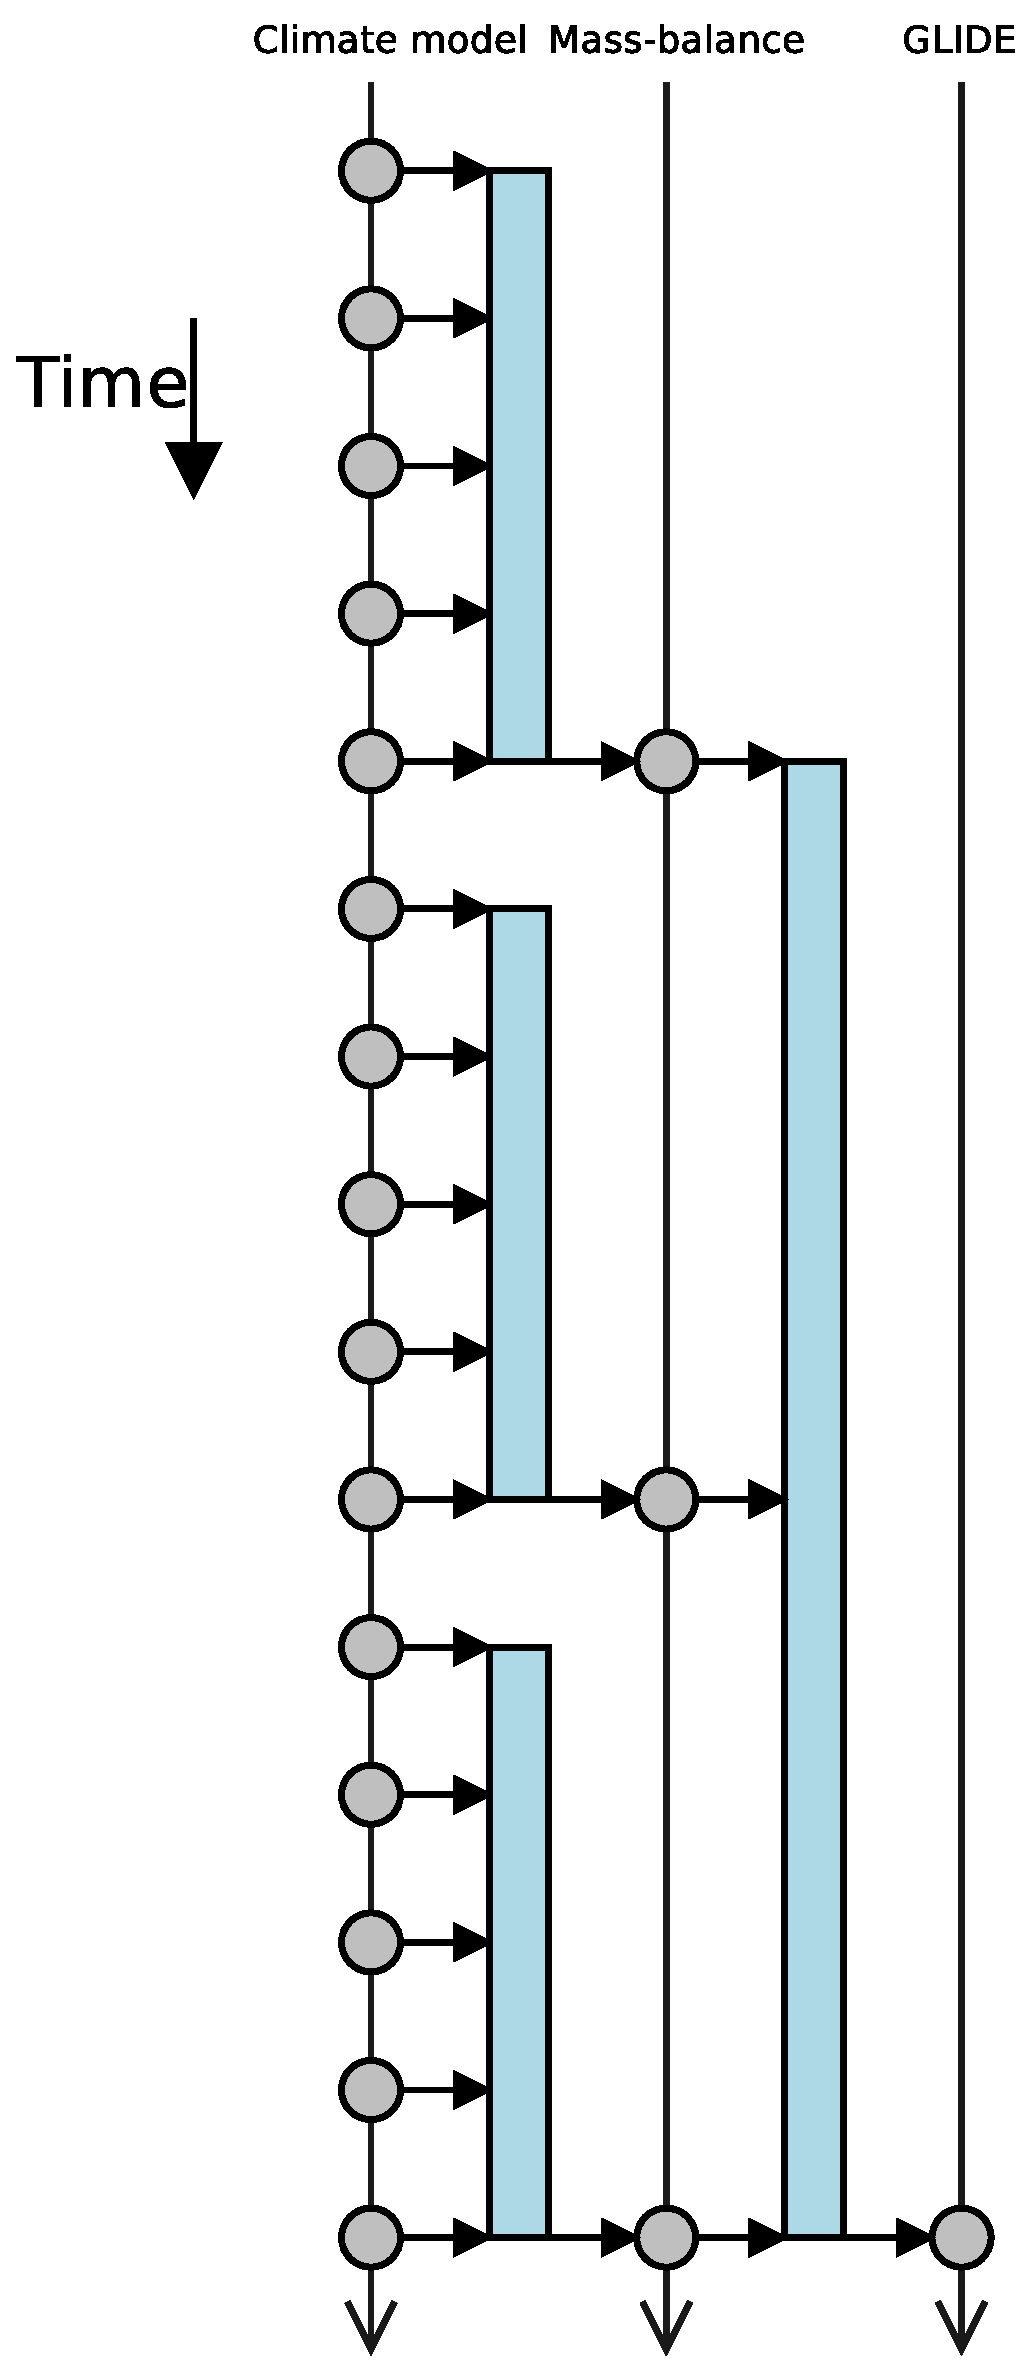
\includegraphics[width=0.6\textwidth]{\dir/figs/glint_timesteps.eps}
  \caption{Relationship between the timesteps in GLINT. The filled circles
  represent timesteps, the rectangles represent averaging/accumulation, and the arrows,
  flow of coupling fields. \textbf{DO WE STILL WANT THIS FIGURE? IS IT STILL ACCURATE?}}
  \label{ug.fig.glint_timesteps}
\end{figure}
%
\subsubsection{Prerequisites}
%
If you plan to use GLINT, the following should be borne in mind:
%
\begin{itemize}
\item Global input fields must be supplied on a latitude-longitude
  grid. The grid does not have to be uniform in latitude, meaning that
  Gaussian grids may be used. Irregular grids (e.g. icosahedral grids) are not
  supported currently. The boundaries of the grid boxes may be specified; if
  not, they are assumed to lie half-way between the grid-points in lat-lon space.
\item In the global field arrays, latitude must be indexed from north to south
  -- i.e. the first row of the array is the northern-most one. Again, some
  flexibility might be introduced into this in the future.
\item The global grid must not have grid points at either of the
  poles. This restriction is not expected to be permanent, but in the meantime
  can probably be overcome by moving the location of the polar points to be
  fractionally short of the pole (e.g. at 89.9$^{\circ}$ and -89.9$^{\circ}$).
\end{itemize}
%
\subsubsection{Initialising and calling}

The easiest way to learn how GLINT is used is by way of an
example. GLINT should be built automatically as part of GLIMMER, and we assume
here that this has been achieved successfully.

Typically, GLINT will be called from the main program body of a
climate model. To make this possible, the compiler needs to be told to use the
GLINT code. Use statements appear at the very beginning of f90 program
units, before even \texttt{implicit none}:
%
\begin{verbatim}
  use glint_main
\end{verbatim}
%
The next task is to declare a variable of type \texttt{glint\_params}, which
holds everything relating to the model, including any number of ice-sheet
instances:
%
\begin{verbatim}
  type(glint_params) :: ice_sheet
\end{verbatim}
%
Before the ice-sheet model may be called from the climate model, it must be
initialised. This is done with the following subroutine call:
%
\begin{verbatim}
  call initialise_glint(ice_sheet,lats,lons,time_step,paramfile)
\end{verbatim}
%
In this call, the arguments are as follows:
%
\begin{itemize}
\item \texttt{ice\_sheet} is the variable of type \texttt{glint\_params}
 defined above;
\item \texttt{lats} and \texttt{lons} are one-dimensional arrays giving the
  locations of the global grid-points in latitude and longitude, respectively;
\item \texttt{time\_step} is the intended interval between calls to GLINT, in
hours. This is known as the \emph{forcing timestep}. 
\item \texttt{paramfile} is the name of the GLINT configuration file.
\end{itemize}
%
The contents of the configuration file will be dealt with later. Having
initialised the model, it may now be called as part of the main climate
model time-step loop:
%
\begin{verbatim}
    call glint(ice_sheet,time,temp,precip,orog)
\end{verbatim} 
%
The arguments given in this example are the compulsory ones only; a large number of
optional arguments may be specified -- these are detailed in the reference
section below. The compulsory arguments are:
%
\begin{itemize}
\item \texttt{ice\_sheet} is the variable of type \texttt{glint\_params}
 defined above;
\item \texttt{time} is the current model time, in hours;
\item \texttt{temp} is the daily mean $2\,\mathrm{m}$ global air temperature field, in
  $^{\circ}\mathrm{C}$;
\item \texttt{precip} is the global daily accumulated precipitation field,
  in $\mathrm{mm}$ (water equivalent, making no distinction
  between rain, snow, etc.);
\item \texttt{orog} is the global orography field, in $\mathrm{m}$.
\end{itemize}
%
Two mass-balance schemes, both based on the positive degree day (PDD) method,
are supplied with GLIMMER, and are available through GLINT. One of these calculates the mass-balance for the
whole year (the \emph{Annual PDD scheme}), while the other calculates on a
daily basis (the \emph{Daily PDD scheme}). The annual scheme incorporates a
stochastic temperature variation to account for diurnal and other variations,
which means that if this scheme is to be used, GLINT should be called such
that it sees a seasonal temperature variation which has had those variations
removed. In practice, this means calling GLINT on a monthly basis, with
monthly mean temperatures. For the daily scheme, no such restriction exists,
and the scheme should be called at least every 6 hours.
%
\subsubsection{Finishing off}
%
After the desired number of time-steps have been run, GLINT may have some
tidying up to do. To accomplish this, the subroutine \texttt{end\_glint}
must be called:
%
\begin{verbatim}
  call end_glint(ice_sheet)
\end{verbatim}
%
\subsubsection{API}
%
A detailed description of the GLINT API may be found in the appendices.
%
\subsubsection{Configuration}
%
GLINT uses the same configuration file format as the rest of GLIMMER. In the
case where only one GLIDE instance is used, all the configuration data for
GLINT and GLIDE can reside in the same file. Where two or more instances are
used, a top-level file specifies the number of model instances and the name of
a configuration file for each one. Possible configuration sections specific to
GLINT are as follows:
\begin{center}
  \tablefirsthead{%
    \hline
  }
  \tablehead{%
    \hline
    \multicolumn{2}{|p{0.98\textwidth}|}{\emph{\small continued from previous page}}\\
    \hline
  }
  \tabletail{%
    \hline
    \multicolumn{2}{|r|}{\emph{\small continued on next page}}\\
    \hline}
  \tablelasttail{\hline}
  \begin{supertabular}{|l|p{11cm}|}
%%%% 
    \hline
    \multicolumn{2}{|l|}{\texttt{[GLINT]}}\\
    \hline
    \multicolumn{2}{|p{0.98\textwidth}|}{Section specifying number of instances.}\\
    \hline
    \texttt{n\_instance} & (integer) Number of instances (default=1)\\
    \hline
%%%% 
    \hline
    \multicolumn{2}{|l|}{\texttt{[GLINT instance]}}\\
    \hline
    \multicolumn{2}{|p{0.98\textwidth}|}{Specifies the name of an
    instance-specific configuration file. Unnecessary if we only have one
    instance whose configuration data is in the main config file.}\\
    \hline
    \texttt{name} & Name of instance-sepcific config file (required).\\
    \hline
%%%% 
    \hline
    \multicolumn{2}{|l|}{\texttt{[GLINT climate]}}\\
    \hline
    \multicolumn{2}{|p{0.98\textwidth}|}{GLINT climate configuration}\\
    \hline
    \texttt{evolve\_ice} & {\raggedright
      specify whether or not the ice sheet evolves in time: \\
      \begin{tabular}{lp{10cm}}
        0 &  Do not evolve ice sheet (hold fixed in time)\\
        {\bf 1} & Allow the ice sheet to evolve \\
      \end{tabular}}\\
    \texttt{precip\_mode} & {\raggedright
      Method of precipitation downscaling: \\
      \begin{tabular}{lp{10cm}}
        {\bf 1} & Use large-scale precipitation rate\\
        2 & Use parameterization of \emph{Roe and Lindzen}\\
      \end{tabular}}\\
    \texttt{acab\_mode} & {\raggedright
      Mass-balance model to use:\\
      \begin{tabular}{lp{7cm}}
        {\bf 1} & Annual PDD mass-balance model (see section \ref{ug.mbal.pdd_scheme}) \\
        2 & Annual accumulation only\\
        3 & Hourly energy-balance model (RAPID - not yet available) \\
        4 & Daily PDD mass-balance model (no docs yet)\\
      \end{tabular}}\\
    \texttt{ice\_albedo} & Albedo of ice --- used for coupling to climate
    model (default=0.4) \\
    \texttt{lapse\_rate} & Atmospheric temperature lapse-rate, used to correct
    the atmospheric temperature onto the ice model orography. This should be
    \emph{positive} for temperature falling with height
    ($\mathrm{K}\,\mathrm{km}^{-1}$) (default=8.0) \\
    %%%%%%%%%%%%%%
    \texttt{data\_lapse\_rate} & Atmospheric temperature vertical lapse rate,
    to be used in the calculation of temperature at
    sea-level. The variable \texttt{lapse\_rate} is then used to adjust the
    temperature to the surface of the local ice sheet topography. If
    \texttt{data\_lapse\_rate} is not set, it is set to the value of
    \texttt{lapse\_rate} by default. \\
    %%%%%%%%%%%%%%
    \texttt{ice\_tstep\_multiply} & Ice time-step multiplier: allows
    asynchronous climate-ice coupling. See below for full explanation of GLINT
    time-stepping. (default = 1) \\
    %%%%%%%%%%%%%%
    \texttt{mbal\_accum\_time} & Mass-balance accumulation time (in years,
    default is equal to mass-balance timestep).  See below for full explanation of GLINT
    time-stepping. \\
    \hline
  \end{supertabular}
\end{center}

\subsubsection{GLINT timestepping --- an explanation}

By default, the model accepts input on each forcing timestep (as specified in 
the call to \texttt{initialise\_glint}, above). These are accumulated over the course 
of a mass-balance time-step, whereupon the mass-balance model is called. The 
output from the mass-balance model is accumulated over the course of an ice 
model time-step, and finally the ice model is called.

This default behaviour can be altered, in two ways:
\begin{enumerate}
\item The number of ice sheet time-steps executed for each accumulated 
mass-balance field may be increased - thus accelerating the icesheet relative 
to the forcing. To do this, set \texttt{ice\_tstep\_multiply} in the \texttt{[GLINT climate]} 
config section - must be an integer. This is only possible if the 
mass-balance is accumulated over an integer number of years.
\item The mass-balance accumulation period can be altered by setting  
\texttt{mbal\_accum\_time} in the \texttt{[GLINT climate]} config section --- this is a 
floating-point value in years.
\end{enumerate}

The interaction of these two parameters is fairly complex, and permits a 
reasonably sophisticated control of how the ice sheet model is forced. 
Various checks are made at run-time to make sure sensible/possible values are selected. Most 
importantly, all relevant time-steps must divide into one another 
appropriately - the model will (should\ldots) stop if an un-sensible combination 
of values is detected.

\subsubsection{GLINT timestepping --- further examples}

To aid understanding of the time-stepping controls, here are some examples. First, suppose we have these time-step values:

\vspace{0.5cm}
\begin{tabular}{ll}
forcing time-step: & 6 hours \\
mass-balance time-step: & 1 day \\
ice time-step: & 0.5 year
\end{tabular}
\vspace{0.5cm}

By default, the model will accumulate 6 months' worth of mass-balance 
calculations, and force the ice sheet model based on that. This might not be 
desirable, so you could set:

\begin{verbatim}
    mbal_accum_time = 1.0
\end{verbatim}

This would make GLINT accumulate 1 year's worth of mass-balance output before 
forcing the ice sheet (at which point it would execute \emph{two} ice sheet 
time-steps of 0.5 years each).

Having done that, you could accelerate the ice model by a factor of ten, by 
setting:

\begin{verbatim}
    ice_tstep_multiply = 10
\end{verbatim}

In this scenario, 20 ice sheet time-steps of 0.5 years each would be done 
after each 12-month accumulation of mass-balance data.

For the second example, we consider the contrasting situation where we don't want to calculate a 
mass-balance on all the available data (perhaps to save time). Consider 
these time-step values:

\vspace{0.5cm}
\begin{tabular}{ll}
forcing time-step:   &   6 hours \\
mass-balance time-step: & 1 day \\
ice time-step:       &   10 years
\end{tabular}
\vspace{0.5cm}

(Clearly this a fairly numerically stable and/or low-resolution ice sheet).

To avoid running the daily PDD scheme c.3600 times (depending on the value of 
\texttt{days\_in\_year}), we can set to only use the first two years of data:

\begin{verbatim}
    mbal_accum_time = 2.0
\end{verbatim}

GLINT accumulates mass-balance for 2 years, then waits for 8 years (incoming 
data are ignored during this time), before calling the ice sheet. Ice sheet 
acceleration may be enabled with \texttt{ice\_tstep\_multiply} as before.

%________________________________________________
%________________________________________________
%
%   GLINT example described here
%________________________________________________
%________________________________________________


\section{GLINT: using glint-example}
If finally you want to see what GLIMMER can do using the GLINT climate driver,
download the \texttt{glint-example} and try one of the provided example setups.
CD into the directory and try any of the config examples. Start glint\_example
by typing
\begin{verbatim}
    glint_example
\end{verbatim}
You will then be asked for a climate configuration file and an ice model 
configuration file.
For the climate file, a global example including precipitation and temperature timeseries
is provided. To let glint know about it, type
\begin{verbatim}
    glint_example.config
\end{verbatim}
For the ice model config, there are two examples, Greenland and North America. To chose either one, type
\begin{verbatim}
  gland20.config
\end{verbatim}
or
\begin{verbatim}
  namerica20.config
\end{verbatim}
respectively at the prompt asking for the config file, to start the model.
Both models are outputting three files each, containing different variables.
Every 100 years, a file \texttt{namerica20.hot.nc} or \texttt{gland20.hot.nc}, respectively is output, 
which can be used to hotstart the model later from any of the recorded stages.

As mentioned above, the model type (binary) to use can be stated in the configuration file,
or given using the \texttt{-m} option. Currently, the three model binaries that
come with GLIMMER are \texttt{simple\_glide, eis\_glide} and
\texttt{glint\_example}. The simple\_glide and eis\_glide drivers that are started using the glide\_launch.py Python script,
which needs to know which binary to address. The model binary can also be set as an environment variable \$GLIDE\_MODEL. 
However, as glint is called directly using the compiled binary \texttt{glint\_example} here, it is not necessary to further 
specify the model.


%________________________________________________
%________________________________________________
%
%   Surface Mass Balance and PDD schemes described here
%________________________________________________
%________________________________________________


\section{Supplied mass-balance schemes}

** We don't use these for anything, and I don't know if any one of us knows about them in any detail. Have we tested them at all recently? If we aren't familiar with them
perhaps we should not support them? **

\subsection{Overview}
The user is, of course, free to supply their own mass-balance model for use
with GLIDE. However, GLIMMER includes within it a annual positive-degree-day model
for mass balance, shortly to be augmented by a similar daily model and an
hourly energy balance model. This section gives details of how to configure
and call these models.
\subsection{Annual PDD scheme}
\label{ug.mbal.pdd_scheme}
The annual PDD scheme is contained in the f90 module \texttt{glimmer\_pdd},
and the model parameters are contained in the derived type
\texttt{glimmer\_pdd\_params}. Configuration data is contained in a standard
GLIMMER config file, which needs to be read from file before initialising the
mass-balance model. The model is initialised by calling the subroutine
\texttt{glimmer\_pdd\_init}, and the mass-balance may be calculated annually
by calling \texttt{glimmer\_pdd\_mbal}. 

\subsubsection{Example of use:}
\begin{verbatim}
  use glimmer_pdd
  use glimmer_config

  ...

  type(glimmer_pdd_params) :: pdd_scheme
  type(ConfigSection),pointer :: config

  ...

  call glimmer_pdd_init(pdd_scheme,config)

  ...

  call glimmer_pdd_mbal(pdd_scheme,artm,arng,prcp,ablt,acab)
\end{verbatim}
In the subroutine call to \texttt{glimmer\_pdd\_mbal}, apart from the
parameter variable \texttt{pdd\_scheme}, there are three input fields
(\texttt{artm}, \texttt{arng} and \texttt{prcp}), which are, respectively, the
annual mean air temperature, annual temperature half-range, and annual
accumulated precipitation fields. The final two arguments are output fields
--- annual ablation (\texttt{ablt}) and annual mass-balance
(\texttt{acab}). All arrays are of type \texttt{real(sp)}. Temperatures are
degrees Celcius, and precipitation, ablation and mass-balance are measured in
m of water equivalent.
%
%
%
\subsubsection{Day-degree calculation}
%
The greater part of the information held in the \texttt{glimmer\_pdd\_params}
derived type comprises a look-up table (the \emph{PDD table}). The model is
implemented this way for computational efficiency.

The table has two dimensions: mean annual air temperature ($T_a$)
(as the second index) and annual air temperature half range (i.e.,
from July's mean to the annual mean $\Delta T_a$) (as the first
index).  Following \emph{Huybrechts and others} [1991], daily air
temperatures ($T_a^\prime$) are assumed to follow a sinusoidal
cycle
\begin{equation}
    T_a^\prime = T_a + \Delta T_a \cos \left( \frac{2 \pi t}{A}
    \right) + \textbf{R}(0,\sigma)
\end{equation}
where $A$ is the period of a year and $R$ is a random fluctuation
drawn from a normal distribution with mean 0 $^\circ$C and
standard deviation $\sigma$ $^\circ$C. \emph{Huybrechts and
others} [1991] indicate that the number of positive degree days
(D, $^\circ$C days) for this temperature series can be evaluated
as
\begin{equation}\label{pdd}
    D = \frac{1}{\sigma \sqrt{2 \pi}}
    \int\limits_0^A
    \int\limits_0^{T_a^\prime+2.5\sigma}
    T_a \times \exp \left( \frac{-(T_a-T_a^\prime)^2}{2 \sigma^2} \right) dT
    dt
\end{equation}
where $t$ is time.  The table is completed by evaluating this integral using a
public-domain algorithm (Romberg integration), by {\it Bauer} [1961]. The
inner and outer integrals are coded as two subroutines
(\texttt{inner\_integral} and \texttt{pdd\_integrand}), which call the Romburg
integration recursively.

The main parameter needed is the assumed standard deviation of
daily air temperatures, which can be set in the configuration file (the
default is 5 $^\circ $C). 

The positive-degree days are then looked up in the table (as a function of
$T_a$ and $\Delta T_a$). We take care to check that this look up is in done
within the bounds of the table.  The final value of $P$ is determined using
bi-linear interpolation given the four nearest entries in the table to the
actual values of $T_a$ and $\Delta T_a$.

The remainder of the loop completes the calculation of the
ablation and accumulation given this value for $P$.
%
\subsubsection{Mass balance calculation} 
%
We use the following symbols: $a$ is total annual ablation; $a_s$
is potential snow ablation; $b_0$ is the capacity of the snowpack
to hold meltwater by refreezing; the total number of positive
degree days ($D$); day-degree factors for snow and ice ($f_s$ and
$f_i$); and the fraction of snowfall that can be held in the
snowpack as refrozen meltwater ($W_max$). Note that the
day-degree factors have been converted from ice to water
equivalents using the ratio of densities.

 First,
determine the depth of superimposed ice ($b_0$) that would have to
be formed before runoff (mass loss) occurs as a constant fraction
($W_{max}$) of precipitation ($P$)
\begin{equation}
    b_0=W_{max} P.
\end{equation}
Now determine the amount of snow melt by applying a constant
day-degree factor for snow to the number of positive day-degrees
\begin{equation}
    a_s=f_s D.
\end{equation}
We now compare the potential amount of snow ablation with the
ability of the snow layer to absorb the melt.  Three cases are
possible. First, all snow melt is held within the snowpack and no
runoff occurs ($a=0$).  Second, the ability of the snowpack to
hold meltwater is exceeded but the potential snow ablation is
still less than the total amount of precipitation so that
$a=a_s-b_0$. Finally, the potential snow melt is greater than the
precipitation (amount of snow available), so that ice melt ($a_i$)
has to be considered as well.  The total ablation is therefore the
sum of snow melt (total precipitation minus meltwater held in
refreezing) and ice melt (deduct from total number of degree days,
the number of degree days needed to melt all snowfall and convert
to ice melt)
\begin{equation}
    a=a_s + a_i = P - b_0 + f_i \left( D-\frac{P}{f_s} \right).
\end{equation}
We now have a total annual ablation, and can find total net mass
balance as the difference between the total annual precipitation
and the total annual ablation.

Note that this methodology is fairly standard and stems from a
series of Greenland papers by Huybrechts, Letreguilly and Reeh in
the early 1990s.
%
%
%
\subsubsection{Configuration}
The annual PDD scheme is configured using a single section in the
configuration file:
\begin{center}
  \tablefirsthead{%
    \hline
  }
  \tablehead{%
    \hline
    \multicolumn{2}{|p{0.98\textwidth}|}{\emph{\small continued from previous page}}\\
    \hline
  }
  \tabletail{%
    \hline
    \multicolumn{2}{|r|}{\emph{\small continued on next page}}\\
    \hline}
  \tablelasttail{\hline}
  \begin{supertabular}{|l|p{11cm}|}
%%%% 
    \hline
    \multicolumn{2}{|l|}{\texttt{[GLIMMER annual pdd]}}\\
    \hline
    \multicolumn{2}{|p{0.98\textwidth}|}{Specifies parameters for the PDD
    table and mass-balance calculation}\\
    \hline
    \texttt{dx} & Table spacing in the $x$-direction ($^{\circ}$C) (default=1.0)\\
    \texttt{dy} & Table spacing in the $y$-direction ($^{\circ}$C) (default=1.0)\\
    \texttt{ix} & Lower bound of $x$-axis ($^{\circ}$C) (default=0.0)\\
    \texttt{iy} & Lower bound of $y$-axis ($^{\circ}$C) (default=-50.0)\\
    \texttt{nx} & Number of values in x-direction (default=31)\\
    \texttt{ny} & Number of values in x-direction (default=71)\\
    \texttt{wmax} & Fraction of melted snow that refreezes (default=0.6) \\
    \texttt{pddfac\_ice} & PDD factor for ice (m day$^{-1}\,^{\circ}$C$^{-1}$)
    (default=0.008)\\
    \texttt{pddfac\_snow} & PDD factor for snow (m day$^{-1}\,^{\circ}$C$^{-1}$) (default=0.003)\\
  \end{supertabular}
\end{center}
\subsubsection{References}

\noindent Bauer (1961) \emph{Comm. ACM} \textbf{4}, 255.

\noindent Huybrechts, Letreguilly and Reeh (1991) \emph{Palaeogeography,
Palaeoclimatology, Palaeoecology (Global and Planetary Change)}
\textbf{89}, 399-412.

\noindent Letreguilly, Reeh and  Huybrechts (1991) \emph{Palaeogeography,
Palaeoclimatology, Palaeoecology (Global and Planetary Change)}
\textbf{90}, 385-394.

\noindent Letreguilly, Huybrechts  and  Reeh (1991) \emph{Journal of
Glaciology} \textbf{37}, 149-157.
%
%%%%%%%%%%%%%%%%%%%%%%%%%%%%%%%%%%%%%%%%%%%%%%%%%%%%%%%%%%%%%%%%%%%%%%%%%%%%%
% Daily PDD scheme
%%%%%%%%%%%%%%%%%%%%%%%%%%%%%%%%%%%%%%%%%%%%%%%%%%%%%%%%%%%%%%%%%%%%%%%%%%%%%
%
\subsection{Daily PDD scheme}
\label{ug.mbal.daily_pdd_scheme}
The other PDD scheme supplied with GLIMMER is a daily scheme. This is simpler than the annual scheme in that it does not incorporate any stochastic variations. The mass-balance is calculated on a daily basis, given the daily mean temperature and half-range, and assuming a sinusoidal diurnal cycle. Consequently, the firn model is more sophisticated than with the annual scheme, and includes a snow-densification parameterization.
%
\subsubsection{Configuration}
The daily PDD scheme is configured using a single section in the configuration file:
\begin{center}
  \tablefirsthead{%
    \hline
  }
  \tablehead{%
    \hline
    \multicolumn{2}{|p{0.98\textwidth}|}{\emph{\small continued from previous page}}\\
    \hline
  }
  \tabletail{%
    \hline
    \multicolumn{2}{|r|}{\emph{\small continued on next page}}\\
    \hline}
  \tablelasttail{\hline}
  \begin{supertabular}{|l|p{11cm}|}
%%%% 
    \hline
    \multicolumn{2}{|l|}{\texttt{[GLIMMER daily pdd]}}\\
    \hline
    \multicolumn{2}{|p{0.98\textwidth}|}{Specifies parameters for the PDD
    table and mass-balance calculation}\\
    \hline
    \texttt{wmax} & Fraction of melted snow that refreezes (default=0.6) \\
    \texttt{pddfac\_ice} & PDD factor for ice (m day$^{-1}\,^{\circ}$C$^{-1}$)
    (default=0.008)\\
    \texttt{pddfac\_snow} & PDD factor for snow (m day$^{-1}\,^{\circ}$C$^{-1}$) (default=0.003)\\
    \texttt{rain\_threshold} & Temperature above which precipitation is held to be rain ($^{\circ}$C) (default=1.0)\\
    \texttt{whichrain} & {\raggedright
      Which method to use to partition precipitation into rain and snow:\\
      \begin{tabular}{lp{7cm}}
        {\bf 1} & Use sinusoidal diurnal temperature variation \\
        2 & Use mean temperature only\\
      \end{tabular}}\\
    \texttt{tau0} & Snow densification timescale (s) (default=10 years)\\
    \texttt{constC} & Snow density profile factor C (m$^{-1}$) (default=0.0165)\\
    \texttt{firnbound} & Ice-firn boundary as fraction of density of ice (default=0.872)\\
    \texttt{snowdensity} & Density of fresh snow ($\mathrm{kg}\,\mathrm{m}^{-3}$) (default=300.0)\\
  \end{supertabular}
\end{center}


